\documentclass[12pt,twocolumn]{article}
\usepackage[utf8]{inputenc}
\usepackage{graphicx}
\usepackage{amsmath}
\usepackage{booktabs}
\usepackage{geometry}
\usepackage{hyperref}
\usepackage{titlesec}
\usepackage{lipsum} % For generating filler text if needed

\geometry{letterpaper, margin=0.75in}
\hypersetup{colorlinks=true, linkcolor=blue, filecolor=magenta, urlcolor=cyan}

\title{\textbf{Design and Implementation of High-Throughput 175-Tap FIR Filter Architectures}}
\author{Jaden [Last Name] \\ \small Advanced VLSI Design (ECSE 4xxx) \\ \small Rensselaer Polytechnic Institute}
\date{\today}

\begin{document}

\maketitle

\begin{abstract}
% TODO: User Fill In
This report presents a comprehensive design space exploration of 175-tap FIR filter architectures. By analyzing performance metrics such as area (ALMs), power, and $F_{max}$ for seven distinct designs, we demonstrate the throughput advantages of parallel and pipelined structures.
\end{abstract}

\section{Introduction}
% TODO: User Fill In
\lipsum[1]

\section{MATLAB Design Methodology}
% TODO: User Fill In

\subsection{Filter Specification}
\begin{itemize}
    \item \textbf{Type:} Low-Pass Equiripple (Parks-McClellan)
    \item \textbf{Taps:} 175
    \item \textbf{Transition Band:} 0.2$\pi$ to 0.23$\pi$ rad/sample
    \item \textbf{Stopband Attenuation:} $>$ 80 dB
\end{itemize}

\subsection{Quantization and Fixed-Point Analysis}
% Discuss Q1.22 for coefficients, 16-bit input/output, and 49-bit accumulator.

\begin{figure}[h]
    \centering
    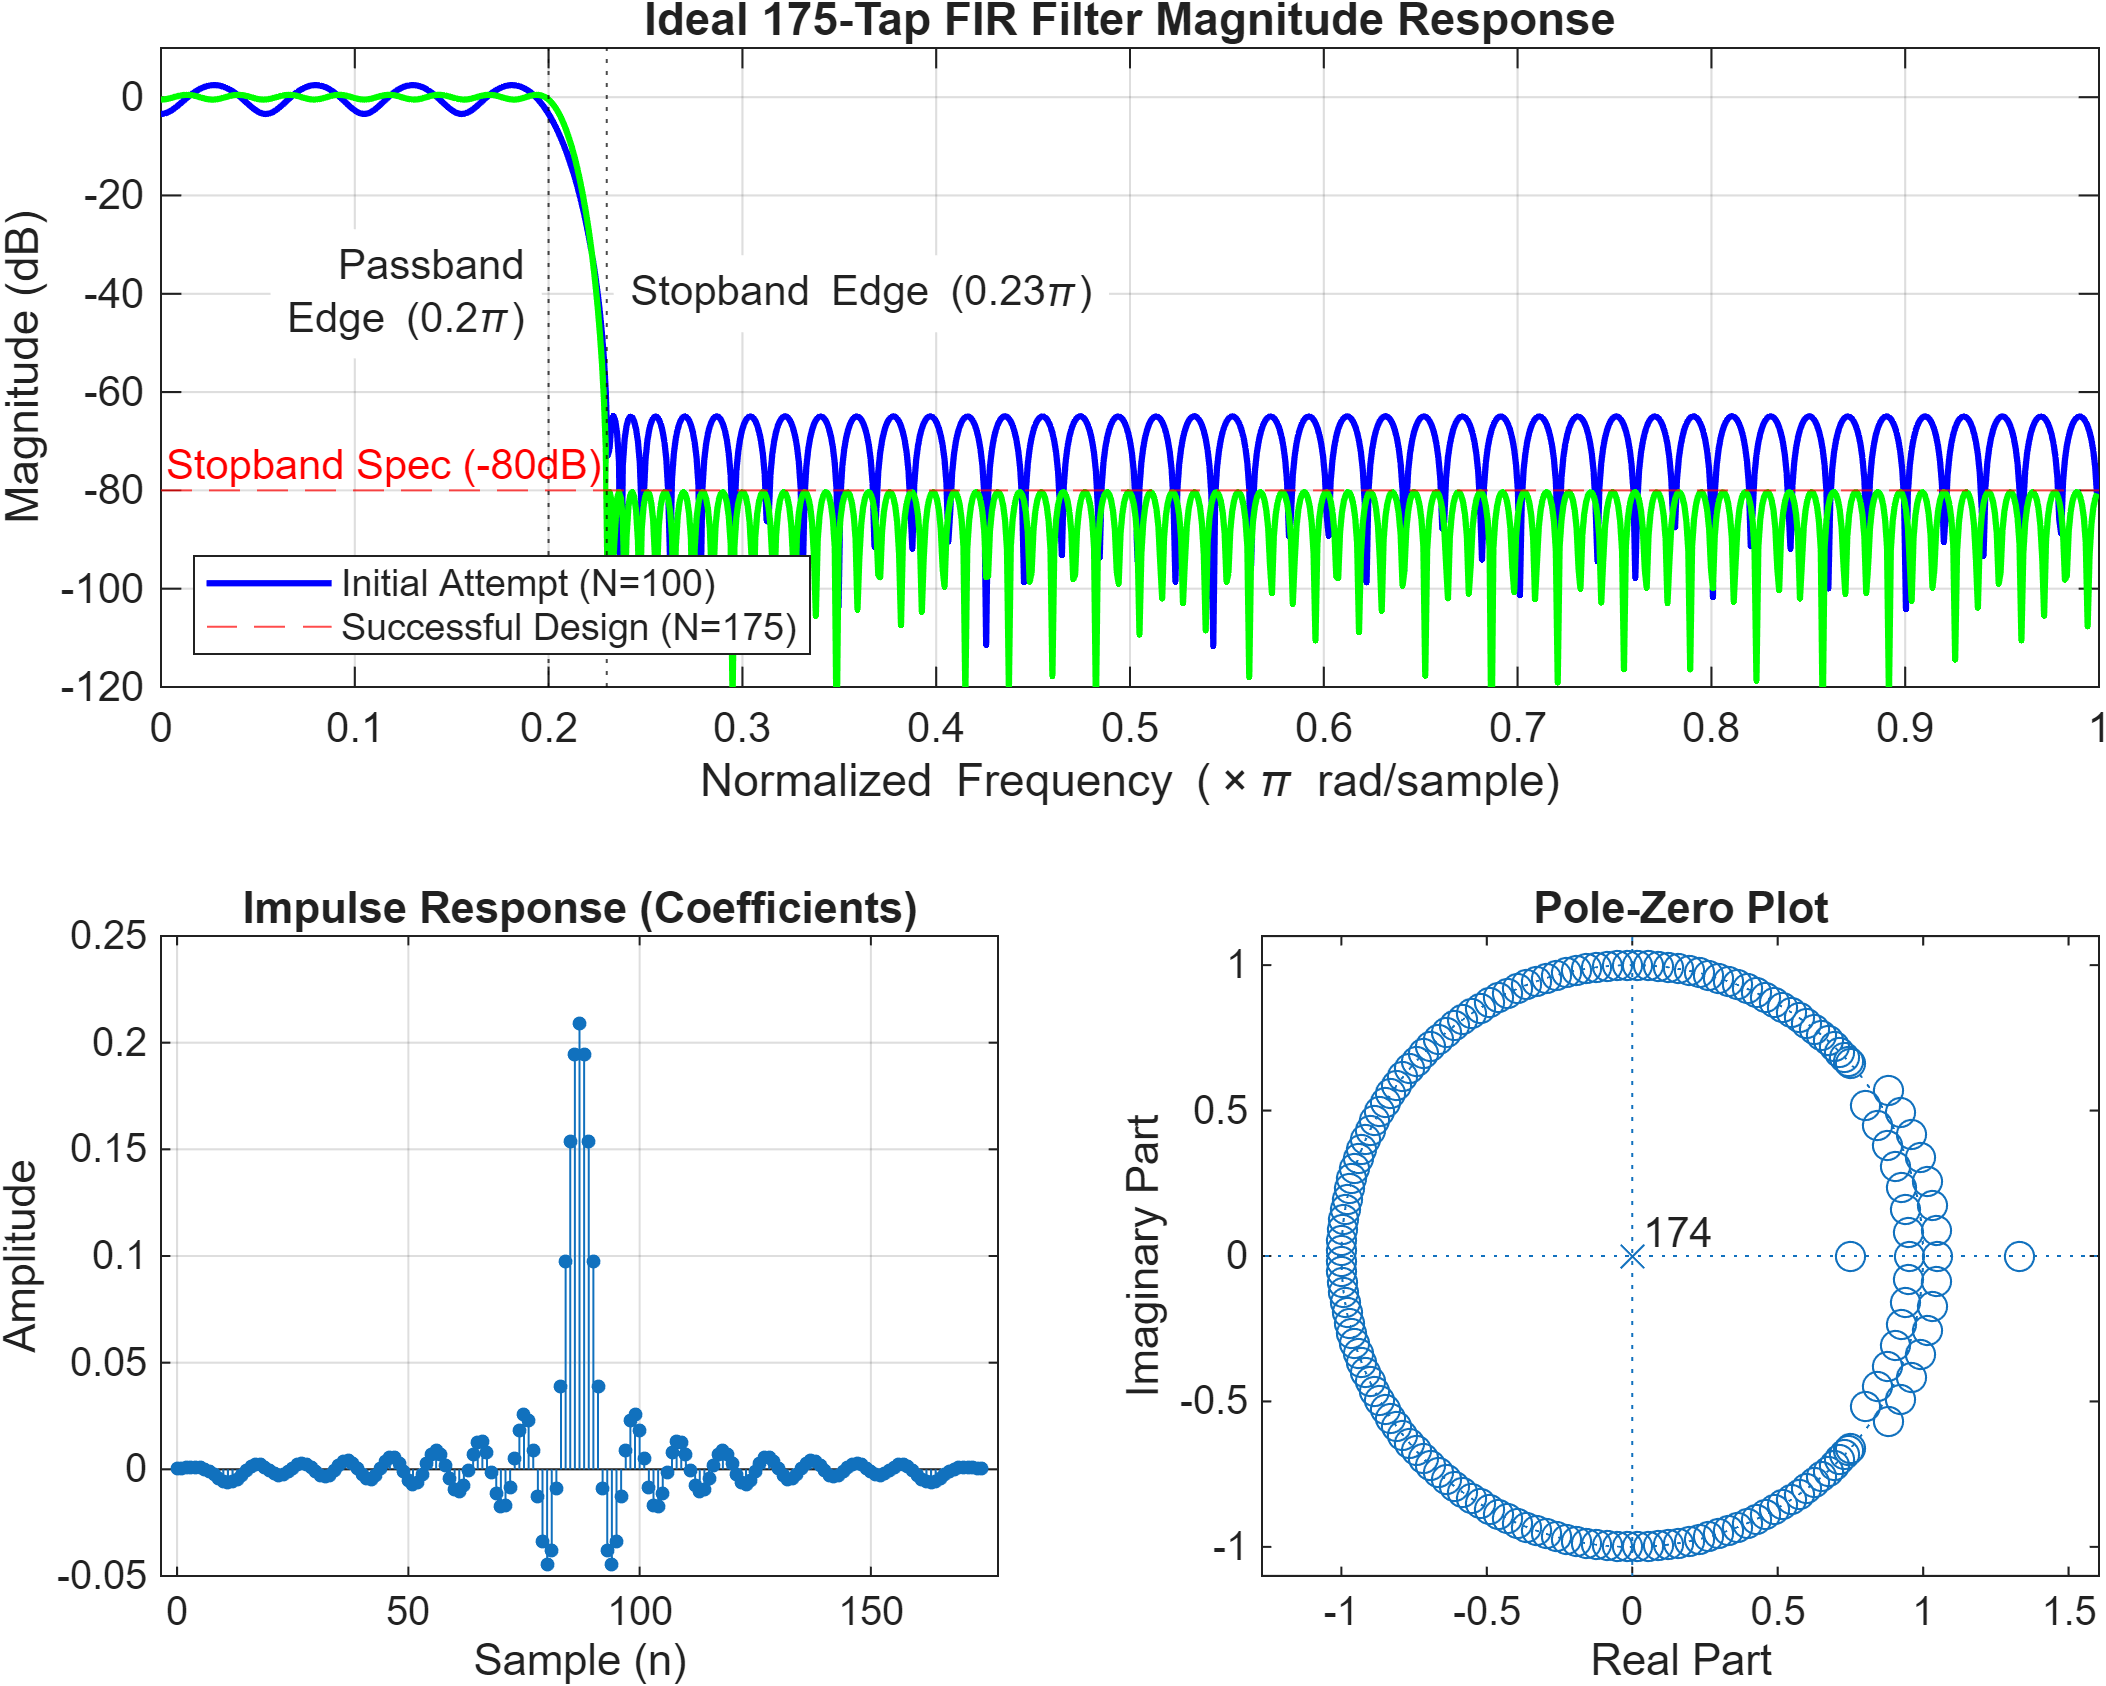
\includegraphics[width=0.95\linewidth]{images/plots/FIR_Filter_Frequency_Response.png}
    \caption{MATLAB frequency response: Original vs. Quantized.}
\end{figure}

\section{Implemented Architectures}
We categorize our seven implementations into four architectural paradigms:

\subsection{Baseline and Pipelined Designs}
% Discuss Direct Form (L=1) and Pipelined FIR.
% Mention the tradeoff between combinational path and cycle latency.

\subsection{Standard Parallel Architectures}
% Discuss L=2 and L=3 Polyphase decomposition.
% Highlight the linear area increase ($N \times L$ multipliers).

\subsection{Reduced-Complexity Parallel (Fast FIR)}
% Discuss the Fast FIR Algorithm (FFA) for L=2 and L=3.
% Cite Mou & Duhamel \cite{mou1991reduced} for the algorithmic reduction.

\subsection{Pipelined Fast FIR (Optimal)}
% Discuss the combination of FFA L=3 with pipelining.

\section{Synthesis Results}
All designs were synthesized and fitted for the Intel Cyclone V FPGA (5CGXFC7C7F23C8) using Quartus Prime Lite.

\begin{table}[h]
\centering
\caption{Hardware Performance Comparison}
\begin{tabular}{@{}lcccc@{}}
\toprule
\textbf{Architecture} & \textbf{ALMs} & \textbf{DSP} & \textbf{$F_{max}$ (MHz)} & \textbf{Power (mW)} \\ \midrule
Direct L=1            & 2,003         & 156          & 34.1                     & 122.56              \\
Pipelined L=1         & 2,016         & 131          & 68.9                     & 93.02               \\
L=2 Parallel          & 14,119        & 156          & 36.8                     & 227.98              \\
L=3 Parallel          & 24,726        & 156          & 35.4                     & 354.13              \\
L=2 Fast FIR          & 18,785        & 0            & 35.4                     & 201.87              \\
L=3 Fast FIR          & 25,604        & 0            & 35.0                     & 302.06              \\
\textbf{Piped FFA L3} & \textbf{14,270} & \textbf{156} & \textbf{68.4}            & \textbf{137.37}     \\ \bottomrule
\end{tabular}
\end{table}

\section{Performance Analysis}
% Discuss Fmax scaling vs Throughput (MSPS = Fmax * L).
% Discuss Area Efficiency and Power Efficiency benchmarks.

\section{Functional Verification}
RTL verification shows bit-exact matches with MATLAB models across all stimuli.

\begin{figure}[h]
    \centering
    % Placeholder for your favorite waveform
    
\includegraphics[width=\linewidth]{images/waveforms/pipelined/full.png}
    \caption{Functional verification: Waveform for [Arch Name].}
\end{figure}

\section{Conclusion}
% TODO: User Fill In
\lipsum[2]

\bibliographystyle{plain}
\bibliography{references}

\end{document}
